\chapter{ПРОЕКТИРОВАНИЕ СИСТЕМЫ УПРАВЛЕНИЯ РОБОТОМ-ГЕКСАПОДОМ}

В данной главе рассматривается этап проектирования управления гексаподом, структура системы управления, подбор технических средств для его реализации, а так же постановка требований, которым должно удовлетворять конечное решение.

\section{Описание системы управления}

На борту гексапода установлен 32 битный ARM–контроллер STM32F100RET6B, который непосредственно, путем подачи необходимого ШИМ – сигнала управляет сервоприводами, установленными в ногах. Принципиальная схема устройства изображена на рисунке \ref{img:principial}

ШИМ – это одно из основных средств, с помощью которых микроконтроллеры управляют аналоговыми устройствами, такими как двигатели с регулируемой скоростью, регулируемые источники света, исполнительные механизмы и динамики. Однако ШИМ не является истинным аналоговым выходом. ШИМ "подделывает" аналогичный результат, применяя мощность в импульсах или коротких импульсах регулируемого напряжения.

Таким образом, подавая ШИМ сигнал различной скважности с контроллера на сервоприводы можно устанавливать определенный угол и тем самым управлять конечностями робота.

\begin{figure}
	\centering
	\includegraphics[width = \linewidth]{img/principial}
	\caption{Принципиальная схема платы управления гексаподом}
	\label{img:principial}
\end{figure}

Для расчетов и генерации походки используется математический пакет ФРУНД – программная система формирования решений уравнений нелинейной динамики. Основной задачей данного пакета является моделирование динамических процессов в машинах и конструкциях. По созданному пользователем описанию расчетной схемы есть возможность создания уравнений математической модели динамики движения исследуемой конструкции, а также генерации программы интегрирования данных уравнений. Решение, обработка и вывод результатов предоставляется в удобной для пользователя форме.

Таким образом, для управления гексаподом применяется статический баланс, при котором, как описывалось ранее, проекция центра масс робота находится в пределах периметра, образованного точками опоры. Генерация алгоритма движения суставов ног производится за помощью пакета ФРУНД, путем решения обратной задачи динамики. В роли исходных параметров выступают траектории движения концов ног робота, и его центра масс.

Для передачи сгенерированных параметров непосредственно в робота используется интерфейс UART – универсальный асинхронный приемник / передатчик – это периферийное устройство микроконтроллера, которое преобразует входящие и исходящие байты данных в последовательный битовый поток. 

Передача по usart осуществляется следующим образом, как показано на рисунке \ref{img:uart}:
\begin{itemize}
	\item В состоянии ожидания вывод трансмиттера находится в положении логической единицы;
	\item Передача байта начинается со стартового бита, который является логическим нулем;
	\item Передача байта оканчивается битом, который является логической единицей;
	\item Передача осуществляется с младшего бита;
	\item В конце может передаваться бит четности (опционально).
\end{itemize}


\begin{figure}[h!]
	\centering
	\includegraphics[width = \linewidth]{img/usart}
	\caption{UART Serial Data}
	\label{img:uart}
\end{figure}

\section{Общая структура системы управления}

На рисунке \ref{img:struct} показана общая структура управления гексаподом

\begin{figure}[]
	\centering
	\includegraphics[width = 0.5\linewidth]{img/struct}
	\caption{Структура системы управления}
	\label{img:struct}
\end{figure}

Оператор задает необходимые параметры для движения и требуемое направление походки в устройстве управления, которое, в свою очередь, формирует их определенным способом для передачи в генератор походки, т.е. ФРУНД посредством использования сокетов.

Сокеты обеспечивают связь между двумя разными процессами на одной и той же машине. Точнее, это способ общения с другими компьютерами с использованием стандартных файловых дескрипторов Unix. В Unix каждое действие ввода / вывода выполняется путем записи или чтения файлового дескриптора. Дескриптор файла - это просто целое число, связанное с открытым файлом, и это может быть сетевое соединение, текстовый файл, терминал или что-то еще.

Генератор походки в данном случае является основным компонентом в системе. Получая данные от устройства управления, выполняется расчет движений для текущего момента времени и управляющий алгоритм для всех суставов робота, которая отправляется непосредственно в гексапод или его эмулятор.

\section {Проектирование системы управления роботом-гексаподом}

Для реализации системы управления необходимо выбрать устройство, благодаря которому будет осуществляться управление. Для начала необходимо выделить необходимые управляющие параметры и их количество. А затем под существующие потребности выбрать наилучший способ реализации интерфейса управления для оператора.

\subsection{Спецификация команд управления}

Реализация команд управления реализована в текстовом пакетном режиме – команды записываются в виде строки вещественных чисел. Пример содержимого в файле сокета команд представлен в таблице \ref{tab:cmdfile}:

\begin{table}[h!]
	\caption{Пример содержимого файла команд}
	\label{tab:cmdfile}
	\begin{tabularx}{\textwidth}{|X|X|X|X|X|X|X|X|X|X|X|X|}
		\tabheader{TS}{DX}{DY}{DZ}{DUX}{DUY}{DUZ}{LST}{HST}{SM}{FB}{GT}
		0.5 	& 5 & 0 & -3 & 0 & 0 & 0 & 0 & 0 & 0 & 0 & 0\\\hline
		2.05 	& 0 & -3 & 0 & 0 & 1 & 0 & 0 & 0 & 0 & 0 & 0\\\hline
		3.15 	& 0 & -3 & 0 & 0 & 0 & 0 & 0 & 0 & 0 & 0 & 2\\\hline
		3.8 	& 0 & -3 & 0 & 1 & 0 & 0 & 0 & 0 & 0 & 0 & 0\\\hline
		19.2 	& -2 & -1 & -3 & 0 & 0 & 0 & 0 & 0 & 0 & 0 & 0\\\hline
		31.4 	& 0 & 0 & 0 & 0 & 0 & 0 & 0 & 0 & 0 & 0 & 0\\\hline
	\end{tabularx}
\end{table}

Значения параметров команд:

\begin{enumerate}
	\item Time stamp;
	\item Величина изменения скорости заданной точки робота в направлении X (условные единицы, значение 1 увеличение (уменьшение -1) скорости на фиксированную величину с фиксированным ускорением, модуль скорости ограничен);
	\item Величина изменения скорости заданной точки робота в направлении Y (условные единицы, аналогичные п. 2);
	\item Величина изменения вертикальной координаты заданной точки робота в направлении Z (условные единицы, значение 1 увеличение (уменьшение -1) высоты на фиксированную величину за фиксированное время, максимальные и минимальные значения ограничены);
	\item Величина изменения угла относительно продольной оси X робота (условные единицы, значение 1 увеличение (уменьшение -1) угла на фиксированную величину за фиксированное время, максимальные и минимальные значения ограничены);
	\item Величина изменения угла относительно поперечной оси Y робота (условные единицы, аналогично п. 5);
	\item Величина изменения угловой скорости робота относительно вертикальной оси Z (условные единицы, значение 1 увеличение (уменьшение -1) скорости на фиксированную величину с фиксированным ускорением, модуль скорости ограничен);
	\item Параметр длины шага - условные единицы, значение 1 увеличение (уменьшение -1) длины шага на фиксированную величину, максимальные и минимальные значения ограничены);
	\item Параметр высоты шага - условные единицы, аналогично п. 8;
	\item Параметр походки — соотношение времени переброса ко времени опоры, аналогично п. 8;
	\item Параметр походки — поперечное расстояние от стопы до кузова, аналогично п. 8;
	\item параметр походки — тип походки — целые числа 1, 2, 3,....
\end{enumerate}

\subsection{Постановка и анализ требований}

В существующей спецификации команд можно выделить главные и второстепенные параметры. Главные параметры нуждаются в постоянном контроле со стороны оператора, т.к. они отвечают за непосредственное перемещение гексапода в пространстве. В данном случае главными будут являться следующие параметры:

\begin{enumerate}
	\item Линейные скорости:
		\begin{itemize}
			\item DX – Величина изменения скорости по оси X;
			\item DY – Величина изменения скорости по оси Y;
			\item DZ – Величина изменения скорости по оси Z.
		\end{itemize}
	\item Угловые скорости:
		\begin{itemize}
			\item DUX – Величина изменения скорости вращения относительно оси X;
			\item DUY – Величина изменения скорости вращения относительно оси Y;
			\item DUZ – Величина изменения скорости вращения относительно оси Z.
		\end{itemize}
\end{enumerate}

Таким образом, к аппаратному устройству управления выделяются следующие требования: пульт должен иметь возможность удобной подстройки всех главных параметров, необходимых для управления гексаподом.
	
Все прочие параметры, а именно:

\begin{itemize}
	\item Параметр длины шага,
	\item Параметр высоты шага,
	\item Параметр отношения времени переброса ко времени опоры,
	\item Параметр поперечного расстояния от стопы до кузова,
	\item Параметр типа походки,
\end{itemize}

названные выше второстепенными, безусловно, тоже являются важными. Но они не нуждаются в постоянном изменении в процессе ходьбы, поэтому в их присутствии на аппаратном пульте нет никакой необходимости.

Следующие требования предъявляются к виртуальному пульту управления:

\begin{itemize}
	\item Возможность управления всеми параметрами;
	\item Интуитивный интерфейс управления;
	\item Адаптивность интерфейса управления;
	\item Возможность использования данного интерфейса на большинстве современных платформ;
	\item Оптимизация интерфейса под устройства с сенсорным экраном;
	\item Синхронизация заданных параметров между устройствами, на которых открыт интерфейс управления.
\end{itemize}
	
\subsection{Проектирование архитектуры системы управления}

В результате проектирования архитектуры системы управления для данного робота-гексапода был получен общий подход, который можно использовать для улучшения данной системы в целом или для построения других аналогичных шагающих роботов и систем управления для них. Разработанная архитектура системы управления изображена на рисунке \ref{img:architecture}.

\begin{figure}[]
	\centering
	\includegraphics[width = \linewidth]{img/architecture}
	\caption{Архитектура системы управления роботом-гексаподом}
	\label{img:architecture}
\end{figure}

При осуществлении управления путем использования "Hardware joystick"{} данные со стиков джойстика передаются по радиочастотам в "Joystick receiver"{}. Далее через USB-USART преобразователь по протоколу IBUS информация о текущем положении стиков джойстика передается в "Joystick receiver bridge"{}. Функциями данного модуля являются прием и обработка параметров. Обработка в данном случае заключается в том, чтобы по определенному алгоритму преобразовать сырые данные, полученные от пульта, к формату интерфейса "Walking params"{}, который ожидает "FRUND bridge"{}.

Если же управление осуществляется через "Web control interface"{} параметры, путем использования http запросов попадают непосредственно на HTTP сервер. Если запущено несколько экземпляров "Web control interface"{} на одном или нескольких устройствах, данные между ними синхронизируются через websocket, дабы избежать той ситуации, что каждый экземпляр будет иметь и передавать свои локальные параметры, которые могут сильно отличаться от других. Аналогично управлению с "Hardware joystick"{} в конечном итоге данные также преобразуются для передачи через интерфейс "Walking params"{} во "FRUND bridge"{}.

Отдельно стоит выделить модуль "FRUND bridge"{}, который преобразует принятые "Walking params"{} к в специальную последовательность, которую ожидает ФРУНД, а затем посредством сокетов через интерфейс "commands"{} передает в него сформированные команды управления. Далее по составленной математической модели робота-гексапода (рис. \ref{img:frund}) ФРУНД генерирует траектории перемещения суставов и также посредством сокетов, используя интерфейс "Joints trajectory"{} передает их обратно во "FRUND bridge"{}.

\begin{figure}[h!]
	\centering
	\includegraphics[width = 0.9\linewidth]{img/frund}
	\caption{Модель робота-гексапода в системе ФРУНД}
	\label{img:frund}
\end{figure}

\begin{figure}[h!]
	\centering
	\includegraphics[width = \linewidth]{img/roscontrol}
	\caption{Пример использования связки GAZEBO +{} ROS +{} ros\_control}
	\label{img:roscontrol}
\end{figure}

Следующим модулем системы является "ROS control"{}, который выделяет следующие интерфейсы для входных параметров: "Joint command"{} и "Joint state"{}. Соответственно "FRUND bridge"{} принимая сгенерированные во ФРУНД траектории должен преобразовать их к определенному формату и передать их, используя данные интерфейсы.

Далее следует довольно стандартная концепция использования пакета "ROS control"{} в связке с GAZEBO и/или аппаратной моделью робота. Обратившись к мануалу можно увидеть следующий обзорный пример (рисунок \ref{img:roscontrol}) взаимосвязи между симуляцией, оборудованием, контроллерами и передачами.

Передача – это элемент в конвейере управления, который трансформирует переменные усилия / потока так, что их продукт – мощность – остается постоянным. Реализация интерфейса передачи отображает переменные усилия / потока на выходные переменные усилия / потока при сохранении мощности.

Таким образом, по умолчанию gazebo\_ros\_control очень прост, хотя его также можно расширить с помощью дополнительной архитектуры плагинов, которая позволяет создавать собственные пользовательские интерфейсы аппаратного обеспечения робота между ros\_control и Gazebo.
 
\section{Обзор решения-аналога}

После изучения некоторого количества публикаций на схожую тематику, была найдена статья "Web-Based Robot Control Interface"{} изданная в журнале "IOP Conference Series: Earth and Environmental Science". В ней авторы рассказывают о создании системы управления для Robotic hand. 

Их архитектура системы состоит из пяти модулей. Серверная часть включает в себя четыре модуля: модуль входа в систему для регистрации пользователя, модуль отображения и управления трехмерной имитационной моделью, модуль последовательной передачи данных, робот и однокристальный модуль. Сторона браузера содержит один модуль: модуль веб-интерфейса управления роботом. Структура показана на рисунке \ref{img:china1}.

\begin{figure}[h!]
	\centering
	\includegraphics[width = \linewidth]{img/china1}
	\caption{Структура решения–аналога}
	\label{img:china1}
\end{figure}

\subsection{Архитектура и сценарий использования}
В работе предполагается следующий сценарий использования: пользователь открывает браузер через компьютер или мобильное устройство. Веб-интерфейс управления роботом открывается при вводе URL-адреса и автоматически переносится в интерфейс входа пользователя. Интерфейс входа в систему имеет ссылку для регистрации, через которую пользователь может получить доступ к странице регистрации. Интерфейс входа и регистрации основан на сервисе PHP5. Поскольку PHP работает на стороне сервера, клиент не может знать конкретную логику кода службы регистрации / входа в систему, который обеспечивает безопасность идентификационной информации. После подтверждения заявки на регистрацию пользователь может войти в систему с именем пользователя и паролем. После получения идентификационной информации пользователя о входе в систему служба входа в систему считывает файл JSON разрешенного белого списка пользователей и проверяет, существует ли полученная пара имени пользователя и пароля в белом списке. Если это так, выполняется переход на веб-интерфейс управления роботом.

Веб-интерфейс управления роботом состоит из JS-модуля отображения имитационной модели, JS-модуля управления соединением на основе ползунка и JS-модуля отображения информации о последовательном порту. Технология WebGL используется для отображения трехмерной модели робота имитационной модели на странице и отслеживания состояния соединения робота. Имитационная модель обновляется в соответствии с изменениями состояния соединения робота. Модуль управления соединением на основе ползунка считывает модель робота, извлекает все соединения робота и создает взаимно-однозначное соответствие между ползунком и соединением. Модуль отображения информации о последовательном порте подписывается на тему данных о последовательном порте. Когда новое сообщение выпущено, модуль анализирует содержимое сообщения и обновляет информацию данных соединений в веб-интерфейсе управления. Когда пользователь перемещает ползунок в интерфейсе управления для генерации действия, код JS считывает новую информацию о соединении и публикует сообщение в теме состояния соединения. После получения сообщения программа имитационной модели ROS обновляет объединенную информацию имитационной модели и отправляет данные в веб-интерфейс, так что имитационная модель веб-интерфейса также изменяется.

ROS-узел управления последовательной связью также подписывается на тему совместного состояния. При получении новой информации о совместном состоянии информация анализируется, и вызывается библиотека Rosserial для записи данных в последовательный порт. Пакет данных последовательно отправляется с помощью кабеля последовательной передачи данных в микроконтроллер, который управляет роботом. Микроконтроллер имеет собственную управляющую логику, позволяющую менять узлы робота, реализовывать дистанционное управление роботом через веб-интерфейс. В то же время узел управления последовательной связью опубликует сообщение о состоянии соединения в разделе с информацией о данных последовательного порта при чтении совместной информации об оборудовании робота из кабеля данных последовательного порта. Модуль JS с информацией о последовательном порте в клиентском веб-интерфейсе управления считывает и анализирует содержимое сообщения. Соединения и значения обновляются в веб-интерфейсе для реализации функции отображения реальной информации о соединениях на стороне робота на клиентском интерфейсе.

Полная архитектура проекта управления роботизированной рукой отражена на рисунке \ref{img:china2}.

\begin{figure}[h!]
	\centering
	\includegraphics[height = 0.9\textheight]{img/china2}
	\caption{Архитектура системы программного обеспечения решения–аналога}
	\label{img:china2}
\end{figure}

\subsection {Анализ и сравнение c предложенным решением}

Решение коллег, безусловно, является очень ценным, хоть и не относится к управлению роботом-гексаподом. Однако принцип который был предложен ими для создания архитектуры системы управления роботизированной рукой, является довольно схожим.

Как можно было понять из описания выше, и скриншоту готовой панели управлении, изображенной на рисунке \ref{img:webhand}, а также по фото совместно с устройством, изображенном на рисунке \ref{img:hand}, веб интерфейс путем использования технологии WebGL отображает все изменения которые должны происходить в ходе обработки команд на имитационной модели в режиме реального времени. Данная опция является очень интересной в визуальном плане и удобной в плане отладки устройства и поиска возможных технических неисправностей, сравнивая движения, выполняемые идеальной виртуальной имитационной и реальной моделями. Поэтому было решено добавить данную возможность в следующих версиях системы для робота-гексапода.

Однако возможность регистрации пользователей и белый список, являются излишними, по крайней мере в данной выпускной работе, потому как аппаратура и ПО не находится в общем доступе. Управление устройством сторонними людьми, не обученными и не компетентными в данной сфере не допускается. Все публичные демонстрационные тесты должны проводиться строго под наблюдением специалистов.

\begin{figure}[h!]
	\centering
	\includegraphics[width = \linewidth]{img/webhand}
	\caption{Robotic hand control UI}
	\label{img:webhand}
\end{figure}

\begin{figure}[h!]
	\centering
	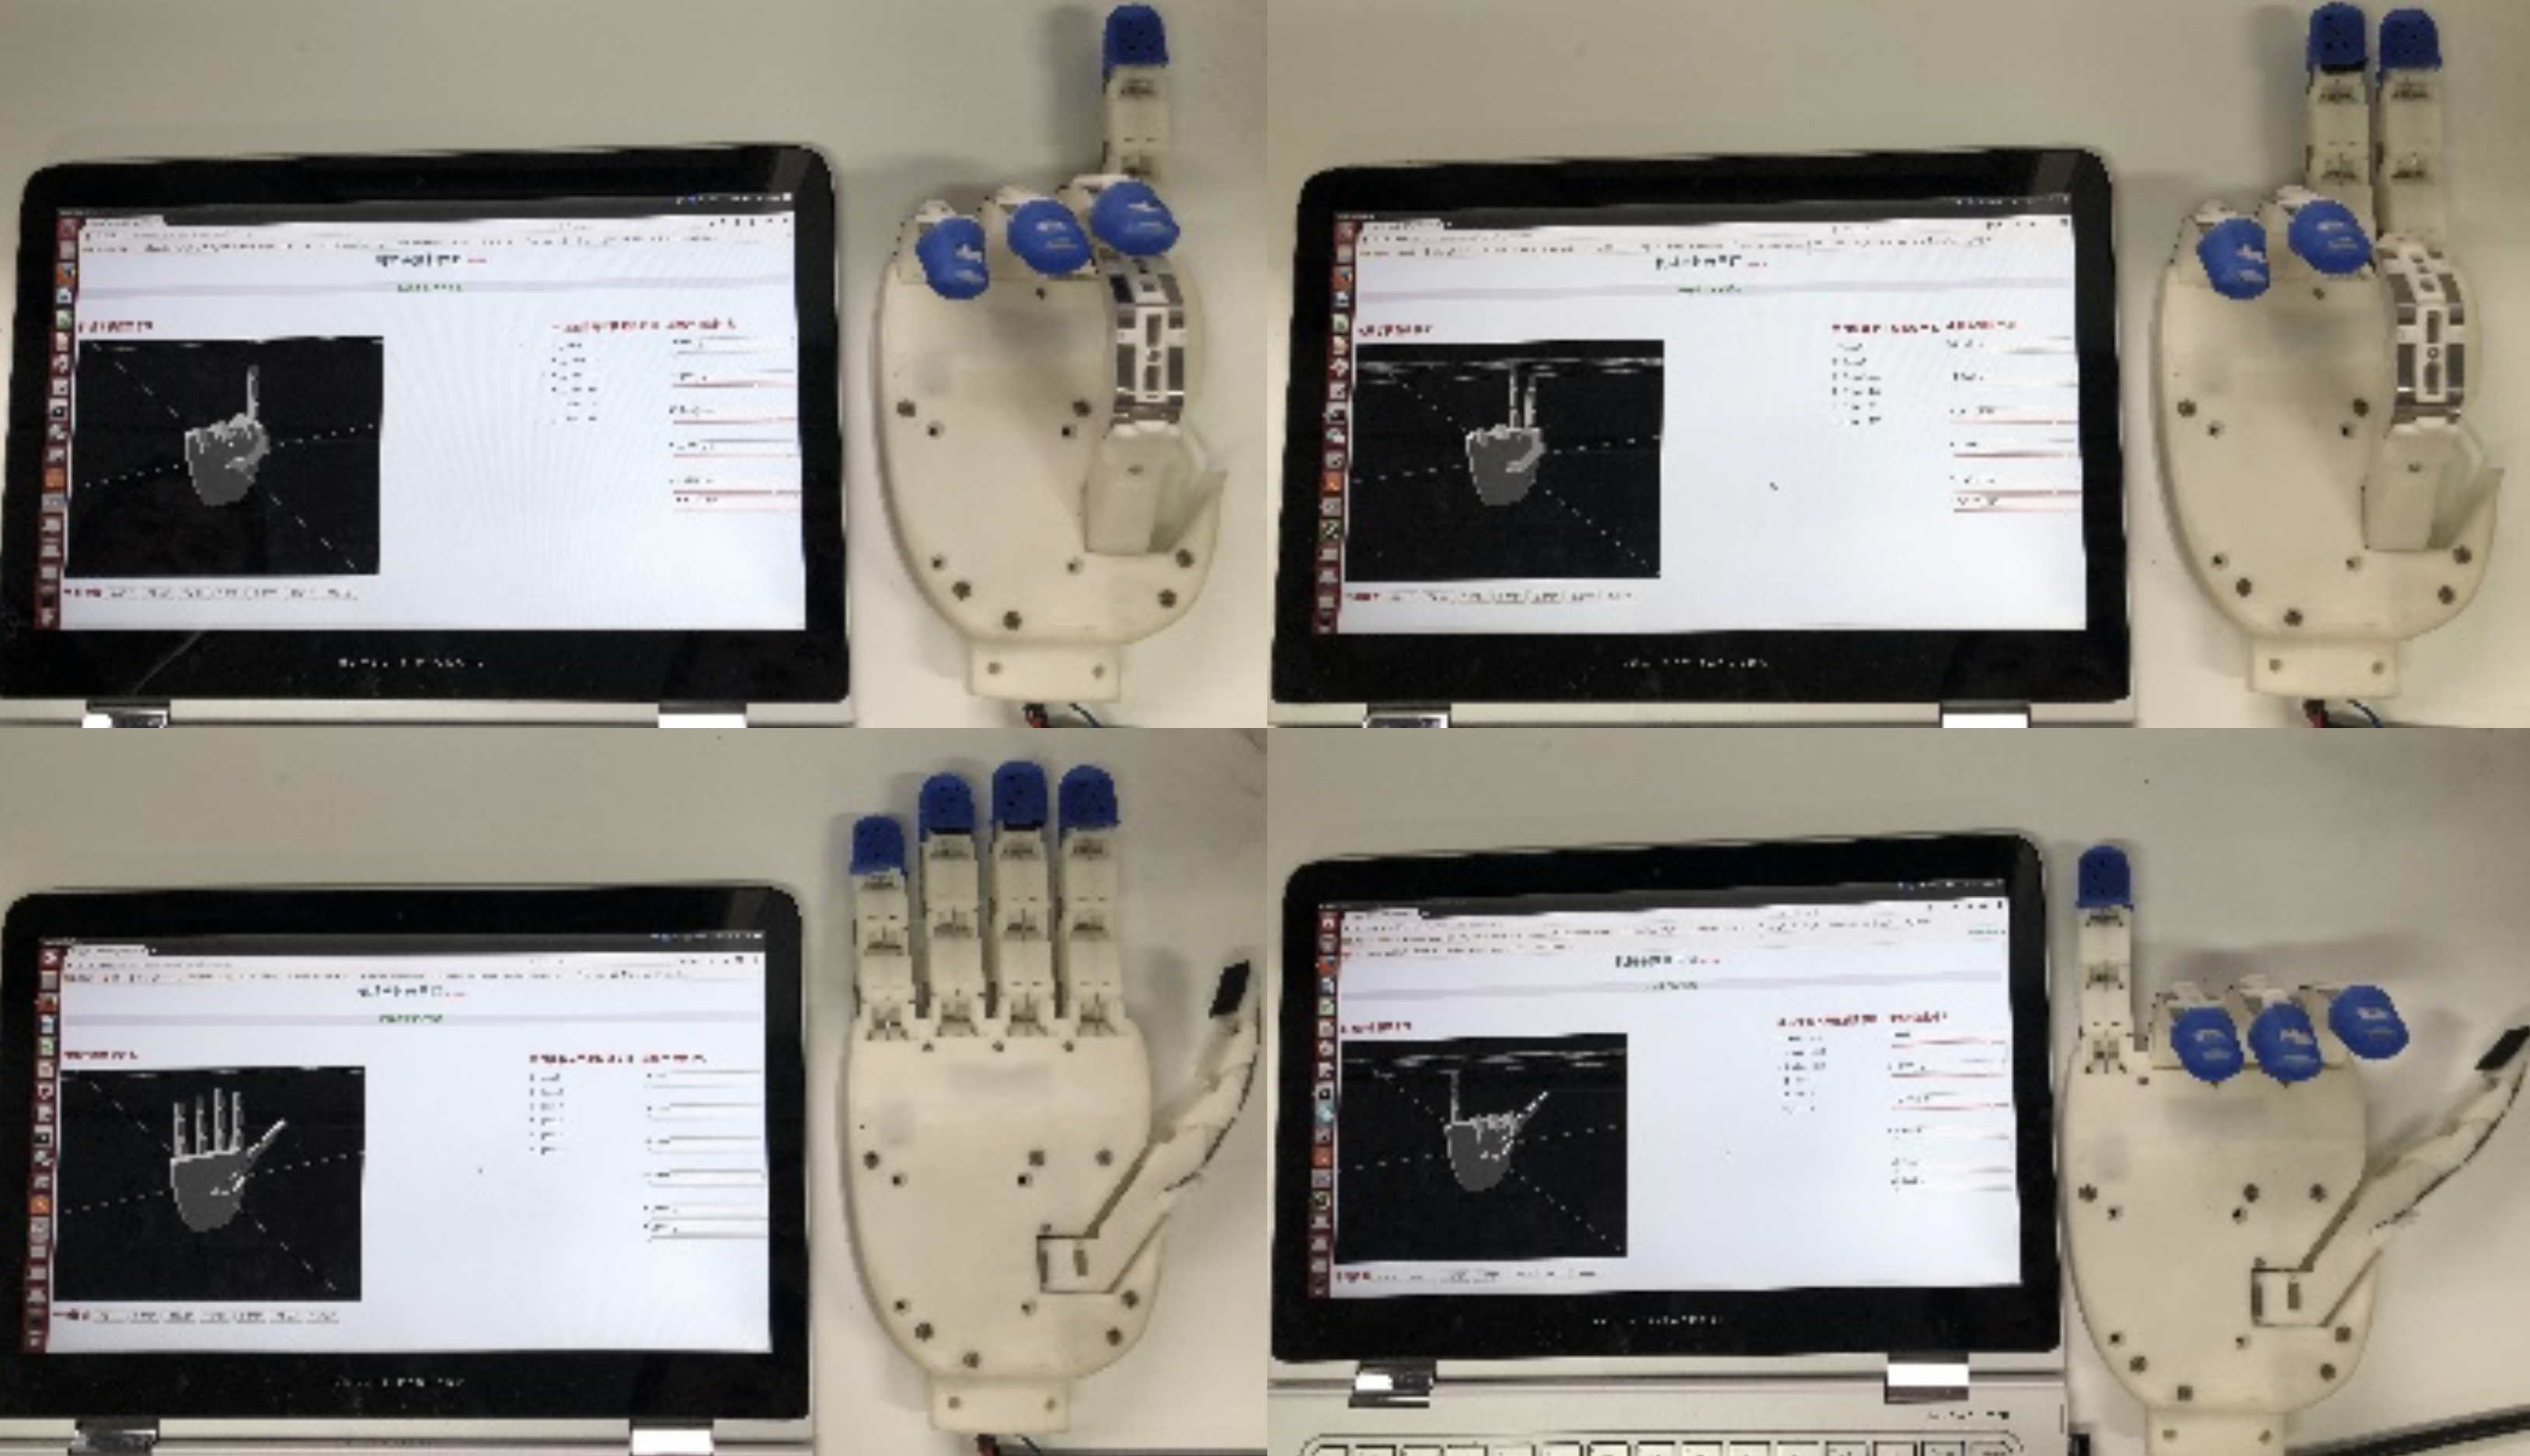
\includegraphics[width = \linewidth]{img/hand}
	\caption{Демонстрация работы системы управления роботизированной рукой}
	\label{img:hand}
\end{figure}

\section{Выводы по главе}

Была разработана общая структура, а также архитектура системы управления роботом-гексаподом с использованием системы ФРУНД, как основного компонента генерации движений. Изучена стандартная архитектура построения систем с использованием пакета ros\_control в связке с ROS и GAZEBO.

Выделены основные критерии и требования разработки системы управления. Рассмотрены плюсы и минусы решения-аналога, которые будут учтены для последующей модернизации решения представленного в третьей главе.

Предложенная концепция использует ROS как связующий слой модулей системы и позволит использовать данное решение для управления новыми моделями робота, а также для модернизации и расширения функционала текущей модели, путем добавления новых программных и аппаратных модулей.